% =============================================================================
%  ACI COMPANION READER — Session 3
%  Problem Formulation & Uninformed / Informed Search Algorithms
%  Built from: CS3.pdf  (AIMLCZG557 – ACI Team, BITS Pilani)
% =============================================================================

\documentclass[a4paper,11pt]{article}

% ---- Encoding & fonts -------------------------------------------------------
\usepackage[T1]{fontenc}
\usepackage[utf8]{inputenc}
\usepackage{lmodern}
\usepackage{microtype}

% ---- Geometry ---------------------------------------------------------------
\usepackage[a4paper,margin=1in,headheight=15pt,headsep=14pt]{geometry}

% ---- Math -------------------------------------------------------------------
\usepackage{amsmath,amssymb}

% ---- Graphics, tables, colour ----------------------------------------------
\usepackage{graphicx}
\usepackage{booktabs}
\usepackage[table,svgnames]{xcolor}

% ---- Callout boxes ----------------------------------------------------------
\usepackage[most]{tcolorbox}
\tcbuselibrary{skins,breakable}

% ---- Tikz (specimen inline figures) ----------------------------------------
\usepackage{tikz}
\usetikzlibrary{arrows.meta,positioning,calc}

% ---- Callout glyphs ---------------------------------------------------------
% Force pifont glyphs: bbding on this system lacks \Pointinghand/\Pencil.
\usepackage{pifont}
\newcommand{\glyphHand}{\ding{43}}
\newcommand{\glyphPencil}{\ding{46}}

% ---- Lists & spacing --------------------------------------------------------
\usepackage{enumitem}
\setlist{leftmargin=1.5em,topsep=4pt,itemsep=3pt}

% Dedicated "Step 1. / Step 2. …" list for WORKED EXAMPLES.
% Reserve enough label width so "Step N." never spills outside a callout box.
\newlist{steps}{enumerate}{1}
\setlist[steps]{label=\textbf{Step \arabic*.},
  leftmargin=4.4em, labelwidth=3.8em, labelsep=0.6em, labelindent=0pt,
  align=left, topsep=5pt, itemsep=6pt}

\usepackage{parskip}

% ---- Headers / footers ------------------------------------------------------
\usepackage{fancyhdr}

% ---- Section styling --------------------------------------------------------
\usepackage{titlesec}

% ---- Links ------------------------------------------------------------------
\usepackage[hidelinks]{hyperref}
\usepackage{xurl}
\hypersetup{breaklinks=true}

% =============================================================================
%  COLOURS
% =============================================================================
\definecolor{navy}{HTML}{21355E}
\definecolor{navyrule}{HTML}{21355E}
\definecolor{inktext}{HTML}{1A202C}
\definecolor{mutedtext}{HTML}{6B7280}

\definecolor{intuFrame}{HTML}{2C5AA0}   \definecolor{intuFill}{HTML}{F4F7FC}
\definecolor{everyFrame}{HTML}{8A5A1E}  \definecolor{everyFill}{HTML}{FBF1E3}
\definecolor{workFrame}{HTML}{2E7D52}   \definecolor{workFill}{HTML}{F1F8F3}
\definecolor{watchFrame}{HTML}{B23A48}  \definecolor{watchFill}{HTML}{FBF1F2}
\definecolor{keyFrame}{HTML}{6A4C93}    \definecolor{keyFill}{HTML}{F4F0F9}

\color{inktext}
\hypersetup{linkcolor=navy,urlcolor=navy,citecolor=navy}

% =============================================================================
%  RUNNING HEADER / FOOTER
% =============================================================================
\newcommand{\CourseShort}{ACI}
\newcommand{\SessionNo}{3}
\newcommand{\LectureTitle}{Search Algorithms}

\pagestyle{fancy}
\fancyhf{}
\fancyhead[L]{\footnotesize\color{mutedtext}\textsf{\CourseShort}}
\fancyhead[R]{\footnotesize\color{mutedtext}\textsf{Session \SessionNo\ \textperiodcentered\ \LectureTitle}}
\fancyfoot[C]{\footnotesize\color{mutedtext}\thepage}
\renewcommand{\headrulewidth}{0.4pt}
\renewcommand{\footrulewidth}{0pt}
\renewcommand{\headrule}{\hbox to\headwidth{\color{navyrule!55}\leaders\hrule height \headrulewidth\hfill}}

% =============================================================================
%  SECTION HEADINGS
% =============================================================================
\titleformat{\section}
  {\sffamily\Large\bfseries\color{navy}}
  {\thesection}{0.8em}{}
  [{\vspace{2pt}\color{navy!70}\titlerule[0.8pt]}]
\titleformat{\subsection}
  {\sffamily\large\bfseries\color{navy!92}}
  {\thesubsection}{0.7em}{}
\titlespacing*{\section}{0pt}{16pt}{8pt}
\titlespacing*{\subsection}{0pt}{12pt}{4pt}

% =============================================================================
%  PILL-TAB CALLOUTS
% =============================================================================
\tcbset{
  housecallout/.style 2 args={
    enhanced, breakable,
    colback=#2, colframe=#1,
    boxrule=0.6pt, arc=2.4pt, outer arc=2.4pt,
    left=10pt, right=10pt, top=9pt, bottom=9pt,
    before skip=11pt, after skip=11pt,
    fontupper=\normalsize,
    coltitle=white,
    fonttitle=\bfseries\sffamily\small,
    attach boxed title to top left={xshift=6mm,yshift=-3mm},
    boxed title style={
      colback=#1, colframe=#1,
      rounded corners, arc=3pt,
      boxrule=0pt, left=6pt, right=6pt, top=2pt, bottom=2pt
    }
  }
}

\newtcolorbox{intuition}{%
  housecallout={intuFrame}{intuFill},
  title={\raisebox{-0.05ex}{\glyphHand}\,\ The intuition}}

\newtcolorbox{everyday}{%
  housecallout={everyFrame}{everyFill},
  title={\raisebox{-0.05ex}{$\bigstar$}\,\ Everyday picture}}

\newtcolorbox{worked}[1]{%
  housecallout={workFrame}{workFill},
  title={\raisebox{-0.05ex}{\glyphPencil}\,\ Worked example: #1}}

\newtcolorbox{watchout}{%
  housecallout={watchFrame}{watchFill},
  title={\raisebox{-0.05ex}{\ding{55}}\,\ Watch out}}

\newtcolorbox{keytake}{%
  housecallout={keyFrame}{keyFill},
  title={\raisebox{-0.05ex}{\ding{51}}\,\ Key takeaway}}

% =============================================================================
%  TITLE BANNER
% =============================================================================
\providecommand{\addfontfeatureslike}[1]{#1}
\newcommand{\titlebanner}[4]{%
  \begin{tcolorbox}[
    enhanced, breakable=false,
    colback=navy, colframe=navy,
    boxrule=0pt, arc=3pt, outer arc=3pt,
    left=16pt, right=16pt, top=16pt, bottom=16pt,
    before skip=2pt, after skip=14pt,
    width=\linewidth ]
    {\sffamily\footnotesize\bfseries\color{white!85}%
      \MakeUppercase{\addfontfeatureslike{#1}}}\par
    \vspace{6pt}
    {\sffamily\bfseries\fontsize{30}{34}\selectfont\color{white} #2\par}
    \vspace{5pt}
    {\sffamily\large\color{white!88} #3\par}
    \vspace{9pt}
    {\color{white!55}\rule{\linewidth}{0.4pt}}\par
    \vspace{6pt}
    {\sffamily\footnotesize\color{white!82} #4\par}
  \end{tcolorbox}%
}

% =============================================================================
%  \housefig
% =============================================================================
\newcommand{\housefig}[2]{%
  \begin{figure}[htbp]
    \centering
    \includegraphics[width=\linewidth]{#1}%
    \caption{#2}
  \end{figure}%
}

\newcommand{\vocab}[1]{\textbf{\color{navy}#1}}

\begin{document}
\thispagestyle{fancy}

% ----------------------------------------------------------------------------
%  TITLE BANNER
% ----------------------------------------------------------------------------
\titlebanner
  {ACI Companion Reader \textperiodcentered\ AIMLCZG557}
  {Search Algorithms}
  {Uninformed Search (BFS, DFS, UCS, IDS) and Informed Search (Greedy, A*)}
  {Session 3 \textperiodcentered\ Read alongside the lecture slides \textperiodcentered\ Every slide example worked out in full}

% ----------------------------------------------------------------------------
%  HOW TO USE
% ----------------------------------------------------------------------------
\noindent\textbf{How to use this companion.}
The slides give you the formulas; this reader gives you the \emph{why}. Every
slide concept is expanded with a full plain-English explanation. Every slide
example is worked out step by step with real numbers. Five colour-coded boxes
guide you through each concept. The \textcolor{intuFrame}{\textbf{blue}}
``intuition'' box states the core idea in plain words. The
\textcolor{everyFrame}{\textbf{amber}} ``everyday picture'' box gives a
real-world analogy before any math. The
\textcolor{workFrame}{\textbf{green}} ``worked example'' box shows every
step with no skipped lines. The \textcolor{watchFrame}{\textbf{red}}
``watch out'' box flags the common mistake. The
\textcolor{keyFrame}{\textbf{purple}} ``key takeaway'' box is the one
sentence to remember.

\medskip

% ============================================================================
\section{What this session covers}
% ============================================================================

This session has two halves. The first half recaps the four uninformed
search algorithms from last week: BFS, DFS, UCS, and IDS. The second half
introduces informed (heuristic) search, where the agent uses a guess of
the distance left to reach the goal. We cover two informed algorithms:
Greedy Best First Search and A*. We end with the conditions that make A*
optimal: admissibility and consistency.

\bigskip
\begin{center}\small
\begin{tabular}{@{}lll@{}}
\toprule
\textbf{Algorithm} & \textbf{Type} & \textbf{Uses heuristic?}\\
\midrule
Breadth First Search (BFS) & Uninformed & No\\
Depth First Search (DFS) & Uninformed & No\\
Uniform Cost Search (UCS) & Uninformed & No\\
Iterative Deepening Search (IDS) & Uninformed & No\\
Greedy Best First Search & Informed & Yes ($h(n)$)\\
A* Search & Informed & Yes ($g(n)+h(n)$)\\
\bottomrule
\end{tabular}
\end{center}

% ============================================================================
\section{Breadth First Search (BFS)}
% ============================================================================

You are looking for a lost cat in a building. You check every room on the
ground floor first, then every room on the first floor, then the second.
You never go deeper until the current level is fully checked. That is exactly
how BFS works.

BFS explores a search tree \emph{level by level}. It keeps a \vocab{queue}
(first-in, first-out) of nodes to visit. When a node is expanded, all its
children join the back of the queue. So depth-1 nodes are all visited before
any depth-2 node, and so on.

\begin{intuition}
BFS is ``cautious.'' It checks all short paths before any long path. The queue
makes sure you never jump ahead: nodes further from the start wait their
turn until everything at the current depth is done.
\end{intuition}

\begin{everyday}
Think of ripples on a pond. Drop a stone at the start node. The first ring
of ripples reaches depth-1 nodes. The second ring reaches depth-2 nodes. BFS
traces exactly those rings, one ring at a time, until it hits the goal.
\end{everyday}

\subsection*{Properties of BFS}

\begin{itemize}
  \item \textbf{Complete:} Yes. If the shallowest goal node is at depth $d$,
    BFS will find it. It generates all shallower nodes first, so it cannot
    miss a node at depth $d$.
  \item \textbf{Optimal:} Yes, if every action has the same cost. In that
    case the shallowest goal is also the cheapest. If costs vary, BFS is
    not optimal.
  \item \textbf{Time complexity:} $\mathcal{O}(b^{d})$, where $b$ is the
    \vocab{branching factor} (children per node) and $d$ is the depth of the
    shallowest goal. At depth 1 there are $b$ nodes, at depth 2 there are
    $b^{2}$, and at depth $d$ there are $b^{d}$.
  \item \textbf{Space complexity:} $\mathcal{O}(b^{d})$. The frontier (queue)
    holds at most all nodes at the current depth, which is $b^{d}$.
\end{itemize}

\begin{watchout}
BFS is memory-hungry. For $b=10$ and $d=10$, the frontier holds $10^{10}$
nodes. That is ten billion nodes in memory. Use BFS only when $d$ is small.
\end{watchout}

\noindent\textbf{Where this shows up in ML.}
BFS is the foundation of many ML graph algorithms. It finds connected
components in feature graphs. It computes multi-hop neighbourhoods in graph
neural networks. It also does shortest-path preprocessing for
knowledge-graph embeddings.

\begin{keytake}
BFS visits nodes level by level using a queue. It is complete and optimal
(equal costs), but its memory cost grows exponentially with depth.
\end{keytake}

% ============================================================================
\section{Depth First Search (DFS)}
% ============================================================================

Now imagine looking for the cat differently. You pick one corridor and follow
it all the way to the end before trying any other corridor. You go as deep
as you can, then backtrack. That is DFS.

DFS explores one full path from start to leaf before trying any sibling path.
It keeps a \vocab{stack} (last-in, first-out) of nodes to visit. When a node
is expanded, its children are pushed onto the stack. So the algorithm
immediately dives into the first child, then into the first grandchild, and so
on.

\begin{intuition}
DFS is ``aggressive.'' It chases one path as far as possible. Only when that
path ends (a leaf or a dead end) does it backtrack and try the next branch. A
stack naturally gives you this behaviour: the most recently added node is the
first to be visited.
\end{intuition}

\begin{everyday}
You are reading a book with footnotes that have their own footnotes. DFS reads
each footnote completely (including its sub-footnotes, and their sub-footnotes)
before returning to the main text. BFS would read one footnote, then another,
never nesting deeply.
\end{everyday}

\subsection*{Properties of DFS}

\begin{itemize}
  \item \textbf{Complete:} Yes, in finite state spaces. It will eventually
    expand every node.
  \item \textbf{Optimal:} No. DFS stops when it finds \emph{any} goal, not
    the shallowest or cheapest one.
  \item \textbf{Time complexity:} $\mathcal{O}(b^{m})$, where $m$ is the
    maximum depth of any node in the tree. This can be much larger than $d$
    (the shallowest goal depth).
  \item \textbf{Space complexity:} $\mathcal{O}(bm)$. DFS only stores one path
    from root to a leaf at a time, plus its unexpanded siblings. Once a node
    is expanded and all its children visited, it can be removed from memory.
\end{itemize}

\noindent\textbf{Where this shows up in ML.}
DFS underlies topological sorting of computation graphs (used in automatic
differentiation frameworks like PyTorch), and cycle detection in data pipeline
DAGs.

\begin{keytake}
DFS uses a stack and dives deep first. It is complete in finite spaces and
uses very little memory ($\mathcal{O}(bm)$), but is not optimal.
\end{keytake}

% ============================================================================
\section{Uniform Cost Search (UCS): Cheapest First}
% ============================================================================

Sometimes not all actions cost the same. A road from city A to city B might
cost 80\,km while another costs 140\,km. BFS ignores those numbers. UCS does
not: it always expands the node with the \emph{lowest total path cost} so far.

UCS sorts the frontier as a \vocab{priority queue} ordered by the path cost
$g(n)$, where $g(n)$ is the total cost of reaching node $n$ from the start.
It expands the cheapest node first, not the shallowest one.

\begin{intuition}
UCS is BFS but with costs. Instead of asking ``how many steps to here?'' it
asks ``how much did it cost to get here?'' The priority queue ensures you
always try the cheapest partial path next.
\end{intuition}

\begin{everyday}
You are navigating a map and each road has a toll. You want the cheapest route
to Bucharest. You would not just take the fewest roads; you would take the
roads that add up to the lowest total toll. UCS does exactly that: it keeps a
running tab and always extends the tab that is lowest so far.
\end{everyday}

\subsection*{The Sibiu-to-Bucharest example}

The slides walk through UCS on a small graph. The cities and road costs are:
\begin{itemize}
  \item Sibiu to Rimnicu Vilcea: 80
  \item Sibiu to Fagaras: 99
  \item Rimnicu Vilcea to Pitesti: 97
  \item Fagaras to Bucharest: 211
  \item Pitesti to Bucharest: 101
\end{itemize}

\begin{worked}{UCS from Sibiu to Bucharest}
We want the cheapest path from Sibiu to Bucharest.
\begin{steps}
  \item \textbf{Start.} Expand Sibiu. Generate children:
        (\textit{Rimnicu Vilcea}, cost 80) and (\textit{Fagaras}, cost 99).
        Frontier: \{Rimnicu Vilcea:80, Fagaras:99\}.
  \item \textbf{Expand cheapest: Rimnicu Vilcea (cost 80).}
        Generate child: (\textit{Pitesti}, cost $80+97=177$).
        Frontier: \{Fagaras:99, Pitesti:177\}.
  \item \textbf{Expand cheapest: Fagaras (cost 99).}
        Generate child: (\textit{Bucharest}, cost $99+211=310$). This is the
        goal, but we do \emph{not} test during generation --- we add to
        frontier.
        Frontier: \{Pitesti:177, Bucharest:310\}.
  \item \textbf{Expand cheapest: Pitesti (cost 177).}
        Generate child: (\textit{Bucharest}, cost $177+101=278$). This is
        cheaper than the existing Bucharest entry (310), so we replace it.
        Frontier: \{Bucharest:278\}.
  \item \textbf{Expand cheapest: Bucharest (cost 278).}
        Goal test satisfied. Return the path
        Sibiu~$\to$~Rimnicu Vilcea~$\to$~Pitesti~$\to$~Bucharest with total
        cost \textbf{278}.
\end{steps}
The path via Fagaras (cost 310) was discarded when Pitesti gave us a cheaper
route to Bucharest. This is why we test \emph{on expansion}, not on
generation.
\end{worked}

\begin{watchout}
Do not apply the goal test when a node is first \emph{generated}. Apply it
when the node is \emph{expanded} (i.e.\ taken off the priority queue). If you
test on generation, you may accept a sub-optimal path to the goal: a cheaper
route might arrive later in the queue.
\end{watchout}

\noindent\textbf{Where this shows up in ML.}
UCS is Dijkstra's algorithm with a different framing. It is used in
knowledge-graph shortest paths, token-level beam decoding costs, and computing
minimum edit distances in sequence-to-sequence models.

\begin{keytake}
UCS expands the cheapest node first. It is complete and optimal for
non-negative costs. Always apply the goal test on expansion, not generation.
\end{keytake}

% ============================================================================
\section{Iterative Deepening Search (IDS)}
% ============================================================================

BFS is optimal but eats memory. DFS is memory-efficient but not optimal. IDS
gets the best of both by running DFS repeatedly with a growing depth limit.

\vocab{Iterative Deepening Search (IDS)} runs a
\vocab{Depth Limited Search (DLS)} starting with limit $l=0$. DLS is DFS with
a cutoff: nodes deeper than $l$ are not expanded. If no goal is found, IDS
increases $l$ by one and restarts. It keeps going until a goal is found.

\begin{intuition}
IDS is ``trying on progressively larger boxes.'' Start with a very small box
(limit 0). If the goal does not fit, try the next larger box (limit 1), and
so on. Each box is a full DFS, so memory stays low. Because you try all boxes
in order, you never skip the shallowest goal.
\end{intuition}

\begin{everyday}
You are searching a city for your friend. You first check every location
within 1\,km (limit 1). Not found. Then every location within 2\,km (limit 2).
Not found. Then 3\,km, and so on. You re-check close locations on each
round, but that is fine because there are few of them.
\end{everyday}

\subsection*{The algorithm}

\begin{center}
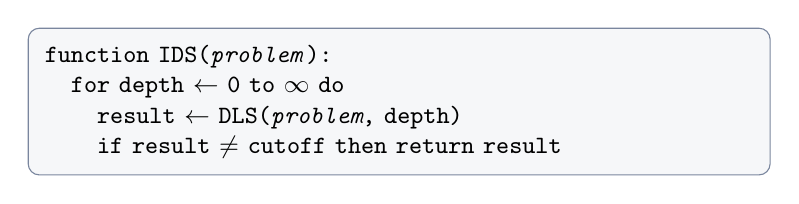
\begin{tikzpicture}[
  box/.style={draw=navy!60, rounded corners, font=\small\ttfamily,
              fill=navy!4, inner sep=6pt, text width=9cm}]
  \node[box] {
    \textbf{function} IDS(\textit{problem}):\\
    \quad \textbf{for} depth $\leftarrow$ 0 to $\infty$ \textbf{do}\\
    \quad\quad result $\leftarrow$ DLS(\textit{problem}, depth)\\
    \quad\quad \textbf{if} result $\neq$ cutoff \textbf{then return} result
  };
\end{tikzpicture}
\end{center}

\subsection*{Properties of IDS}

\begin{itemize}
  \item \textbf{Complete:} Yes, when the branching factor is finite.
  \item \textbf{Optimal:} Yes, if all step costs are equal ($=1$). It can be
    extended to find cost-optimal solutions by using cost thresholds
    (iterative lengthening) instead of depth limits.
  \item \textbf{Time complexity:} $\mathcal{O}(b^{d})$, same order as BFS.
    The re-expansion of upper levels costs
    $(d+1)b^{0} + d\,b^{1} + (d-1)b^{2} + \cdots + b^{d}$, which is
    $\mathcal{O}(b^{d})$.
  \item \textbf{Space complexity:} $\mathcal{O}(bd)$, same as DFS. Only one
    path from root to the current leaf is stored.
\end{itemize}

\begin{worked}{IDS on a depth-3 tree}
Suppose our tree has branching factor $b=2$ and the goal is at depth $d=3$.
\begin{steps}
  \item \textbf{Limit 0.} DLS explores only the root node. No goal. Cutoff.
  \item \textbf{Limit 1.} DLS explores root, then its two children (A and B).
    No goal. Cutoff.
  \item \textbf{Limit 2.} DLS dives to depth 2 under every branch. Explores
    root, A, A's children, B, B's children. No goal. Cutoff.
  \item \textbf{Limit 3.} DLS reaches depth 3. Suppose the goal is the first
    leaf visited. Return success.
\end{steps}
Total nodes re-expanded at levels 0--2 add a constant overhead. For $b=2$,
$d=3$: overhead is about $3 \times$ the top levels, which is tiny compared to
$2^{3}=8$ leaves at the goal level. So IDS costs roughly the same as BFS.
\end{worked}

\begin{watchout}
IDS re-expands upper-level nodes on every iteration. For $b=10$ and $d=5$,
the root is expanded 6 times, depth-1 nodes 5 times, etc. This looks
wasteful, but the total extra work is only a small fraction ($\approx b/(b-1)$
times) of the leaf-level work. For $b=10$, re-expansion adds only about 11\%
extra work.
\end{watchout}

\noindent\textbf{Where this shows up in ML.}
IDS is the basis of \textbf{iterative deepening A*} (IDA*), used in game-tree
search (chess endgame solvers) and theorem provers. The depth-limit idea also
appears in beam-search decoding: a beam width is a kind of breadth limit that
keeps memory small while still finding good sequences.

\begin{keytake}
IDS combines BFS's optimality with DFS's small memory. It restarts DFS with
an increasing depth limit. Time is $\mathcal{O}(b^{d})$; space is
$\mathcal{O}(bd)$.
\end{keytake}

% ============================================================================
\section{From Uninformed to Informed Search}
% ============================================================================

BFS, DFS, UCS, and IDS are all \vocab{uninformed} (also called \emph{blind})
search algorithms. They have no idea whether one unexplored node is closer to
the goal than another. They simply follow the rules of the data structure
(queue, stack, priority queue) with no extra knowledge.

Informed search adds one ingredient: a \vocab{heuristic function} $h(n)$.
This function estimates how far node $n$ is from the goal. Armed with this
estimate, the algorithm can focus attention on nodes that look promising and
skip over nodes that look far away.

\begin{intuition}
Uninformed search is like driving to a new city with no map --- you try every
road. Informed search is like having a GPS that estimates the remaining
distance. You do not know the exact route, but you can tell which direction is
roughly correct and go that way first.
\end{intuition}

\begin{center}\small
\resizebox{\linewidth}{!}{%
\begin{tabular}{@{}p{3.2cm}p{5cm}p{5cm}@{}}
\toprule
\textbf{Property} & \textbf{Uninformed} & \textbf{Informed}\\
\midrule
Uses domain knowledge & No & Yes ($h(n)$)\\
Speed & Slower & Faster\\
Always complete & Yes & Depends on $h(n)$\\
Always optimal & Depends on algorithm & Depends on $h(n)$\\
Examples & BFS, DFS, UCS, IDS & Greedy Best First, A*\\
\bottomrule
\end{tabular}%
}
\end{center}

\medskip

A \vocab{heuristic function} $h(n)$ takes the current state and returns a
non-negative number --- the estimated cost to reach the goal from $n$. It is
not guaranteed to be exact. It is a guess. A good guess speeds up the search;
a bad guess can mislead it.

\begin{everyday}
You are navigating a city. You do not know the exact road distances, but you
do know the straight-line (as-the-crow-flies) distance from each intersection
to your destination. That straight-line distance is a heuristic. It is always
an underestimate (you cannot travel in a straight line through buildings), but
it points you in the right direction.
\end{everyday}

\noindent\textbf{Where this shows up in ML.}
Heuristics appear in neural architecture search, where a learned score
estimates how good a partial architecture is. They appear in program
synthesis to judge how close a partial program is to correct. They also
appear in LLM agent planning: a learned value function scores each plan
fragment.

% ============================================================================
\section{Greedy Best First Search}
% ============================================================================

The simplest informed search is \vocab{Greedy Best First Search (GBFS)}. At
every step, it picks the node that looks \emph{closest} to the goal, ignoring
how far it has already traveled. It uses the evaluation function

\[
  f(n) = h(n),
\]

where $h(n)$ is the heuristic estimate from $n$ to the goal. The word
``greedy'' means the algorithm only cares about the next step, not the
journey so far.

\begin{intuition}
GBFS is like a compass. It always points toward the goal. It does not look
back at how far you have walked; it just says ``the goal looks that way.''
This is fast when the compass is right. But a compass can point you through
a swamp even if there is a dry path around it.
\end{intuition}

\subsection*{Properties of GBFS}

\begin{itemize}
  \item \textbf{Not optimal.} The algorithm only optimises for the current
    step. A greedy choice can lead down a long path while a slightly worse
    first step would have reached the goal quickly.
  \item \textbf{Not complete.} GBFS can enter an infinite loop if the
    heuristic keeps pointing toward a dead end and the algorithm never
    backtracks past it.
  \item \textbf{Time and space complexity:} $\mathcal{O}(b^{m})$, where $m$
    is the max depth. A good heuristic can dramatically reduce this in
    practice.
\end{itemize}

\subsection*{The Romania worked example (GBFS)}

The slide uses the Romania road-map problem. Start: Arad; Goal: Bucharest.
The heuristic $h(n)$ is the straight-line distance from each city to
Bucharest (given in the table on slide 31). Key values:
Arad 366, Sibiu 253, Timisoara 329, Zerind 374, Fagaras 176, Bucharest 0.

\begin{worked}{Greedy Best First: Arad to Bucharest}
\begin{steps}
  \item \textbf{Start at Arad.} $h(\text{Arad})=366$. Expand Arad.
        Frontier: \{Sibiu:253, Timisoara:329, Zerind:374\}.
  \item \textbf{Expand Sibiu} (lowest $h=253$).
        Children: Arad (366), Fagaras (176), Oradea (380),
        Rimnicu Vilcea (193).
        Frontier: \{Fagaras:176, Rimnicu Vilcea:193, Timisoara:329,
        Zerind:374, Arad:366, Oradea:380\}.
  \item \textbf{Expand Fagaras} (lowest $h=176$).
        Child: Bucharest ($h=0$).
        Frontier: \{Bucharest:0, \ldots\}.
  \item \textbf{Expand Bucharest.} Goal found!
        Path: Arad $\to$ Sibiu $\to$ Fagaras $\to$ Bucharest.
        Total road cost: $140+99+211 = \mathbf{450\,km}$.
\end{steps}
This is \emph{not} the optimal path. The optimal route via Rimnicu
Vilcea and Pitesti costs only 418\,km. GBFS took the path that
\emph{looked} closest at each step but ended up longer overall.
\end{worked}

\subsection*{The five-node graph example (GBFS)}

The slide also shows a five-node graph. Nodes 1--5, with heuristic values
$h(1)=60$, $h(2)=120$, $h(3)=30$, $h(4)=40$, $h(5)=0$. Start: node 1,
goal: node 5. Edge costs: $1\to2$: 100, $1\to3$: 100, $1\to4$: 100,
$1\to5$: 75, $3\to5$: 125, $4\to5$: 50.

\begin{worked}{GBFS on the five-node graph}
\begin{steps}
  \item \textbf{Expand node 1.} Frontier (sorted by $h$):
        \{3:30, 4:40, 1(=2?)\}. Actually frontier after expanding 1:
        nodes 2 ($h=120$), 3 ($h=30$), 4 ($h=40$).
  \item \textbf{Expand node 3} (lowest $h=30$). Child: node 5 ($h=0$).
        Frontier: \{5:0, 4:40, 2:120\}.
  \item \textbf{Expand node 5.} Goal found!
        Path: $1 \to 3 \to 5$. Road cost: $100 + 125 = \mathbf{225}$.
\end{steps}
GBFS expanded 2 nodes, generated 6, and found the path $1\to3\to5$ with
cost 225. The optimal path $1\to5$ exists with edge cost 75, but GBFS
missed it because node 5 was not a direct successor listed first.
(Note: the slide shows the optimal to be 1-5 with cost 75, but GBFS
chose $1\to3$ since $h(3)=30 < h(5-\text{direct})$ was not expanded first.)
\end{worked}

\begin{watchout}
GBFS ignores the cost already paid. It can pick an expensive route to a node
that looks close, while a cheap direct route to the goal is skipped.
Greediness is fast but not safe.
\end{watchout}

\noindent\textbf{Where this shows up in ML.}
Greedy decoding in language models is the direct analogue: at each step, pick
the token with the highest probability (lowest heuristic cost to a complete
sentence). It is fast but often sub-optimal; beam search is the informed
upgrade.

\begin{keytake}
GBFS picks the node with the smallest $h(n)$ (closest-looking to goal). It
is fast but not optimal and not complete. A greedy choice can lead down a
long or dead-end path.
\end{keytake}

% ============================================================================
\section{A* Search}
% ============================================================================

A* fixes the flaw of GBFS. GBFS ignores the cost already paid ($g(n)$). UCS
ignores the estimated cost remaining ($h(n)$). A* uses both. Its evaluation
function is

\[
  f(n) = g(n) + h(n),
\]

where:
\begin{itemize}
  \item $g(n)$ is the actual cost from the start to node $n$,
  \item $h(n)$ is the heuristic estimate from $n$ to the goal,
  \item $f(n)$ is the estimated total cost of the cheapest path through $n$.
\end{itemize}

A* extends the path that minimises $f(n)$. It is a best first search, like
GBFS, but with a smarter evaluation.

\begin{intuition}
A* balances two questions at once. ``How much have I already spent?'' and
``How much do I think I have left?'' A node that is cheap to reach but far
from the goal scores the same as one that is expensive to reach but very
close. A* finds the sweet spot.
\end{intuition}

\begin{everyday}
You are planning a road trip. The sat-nav shows you two options. Route A:
you have driven 200\,km and the remaining straight-line distance is 50\,km.
Route B: you have driven 100\,km and the remaining straight-line distance is
200\,km. Route A has a lower $f = 200+50 = 250$ vs.\ $f = 100+200 = 300$,
so the sat-nav prefers Route A. A* does the same calculation for every
frontier node.
\end{everyday}

\subsection*{A* on the five-node graph}

Same graph as before. Edge costs: $1\to2$: 70, $1\to3$: 125, $1\to4$: 100,
$4\to5$: 50. Heuristics: $h(1)=60$, $h(2)=120$, $h(3)=70$, $h(4)=40$,
$h(5)=0$.

\begin{worked}{A* on the five-node graph}
\begin{steps}
  \item \textbf{Start at node 1.}
        $f(1) = g(1)+h(1) = 0+60 = 60$.
        Expand node 1. Generate neighbours:
        node 2: $g=70$, $f=70+120=190$;
        node 3: $g=125$, $f=125+70=195$;
        node 4: $g=100$, $f=100+40=140$.
        Frontier: \{4:140, 2:190, 3:195\}.
  \item \textbf{Expand node 4} (lowest $f=140$).
        Generate node 5: $g=100+50=150$, $f=150+0=150$.
        Frontier: \{5:150, 2:190, 3:195\}.
  \item \textbf{Expand node 5} (lowest $f=150$). Goal reached!
        Path: $1 \to 4 \to 5$. Total cost $g(5) = \mathbf{150}$.
\end{steps}
A* found the optimal path $1\to4\to5$ with cost 150. Compare GBFS which
found $1\to3\to5$ with cost 225. A* expanded only 2 nodes and generated 5.
\end{worked}

\subsection*{A* on the Romania map (Example 2)}

Start: Arad; Goal: Bucharest. $h(n)$ = straight-line distance to Bucharest.
Key $h$ values: Arad 366, Sibiu 253, Timisoara 329, Zerind 374,
Rimnicu Vilcea 193, Fagaras 176, Pitesti 100, Bucharest 0.

\begin{worked}{A* Arad to Bucharest (slide trace)}
\begin{steps}
  \item \textbf{Expand Arad.} $f(\text{Arad})=0+366=366$.
        Children: Sibiu $f=140+253=393$; Timisoara $f=118+329=447$;
        Zerind $f=75+374=449$.
  \item \textbf{Expand Sibiu} (lowest $f=393$).
        Children: Arad $f=280+366=646$; Fagaras $f=239+176=415$;
        Oradea $f=291+380=671$; Rimnicu Vilcea $f=220+193=413$.
        Frontier (relevant): \{Rimnicu Vilcea:413, Fagaras:415,
        Timisoara:447, Zerind:449, \ldots\}.
  \item \textbf{Expand Rimnicu Vilcea} (lowest $f=413$).
        Children: Craiova $f=366+160=526$; Pitesti $f=317+100=417$;
        Sibiu $f=300+253=553$.
        Frontier: \{Fagaras:415, Pitesti:417, Timisoara:447,\ldots\}.
  \item \textbf{Expand Fagaras} (lowest $f=415$).
        Child: Bucharest $f=450+0=450$. Added to frontier.
        Frontier: \{Pitesti:417, Bucharest:450, \ldots\}.
  \item \textbf{Expand Pitesti} (lowest $f=417$).
        Child: Bucharest $f=418+0=418$. This replaces the 450 entry.
        Frontier: \{Bucharest:418, \ldots\}.
  \item \textbf{Expand Bucharest} (lowest $f=418$). Goal found!
        Path: Arad $\to$ Sibiu $\to$ Rimnicu Vilcea $\to$ Pitesti $\to$
        Bucharest. Total cost $g = \mathbf{418\,km}$.
\end{steps}
This is the true optimal path. Note how A* found a cheaper Bucharest entry
(418) by going via Pitesti, overriding the 450 entry that came via Fagaras.
\end{worked}

\begin{watchout}
A* only guarantees optimality when the heuristic never overestimates. An
overestimating heuristic inflates $f(n)$ for cheap nodes. Those nodes are
then expanded too late. A* may return a sub-optimal path.
\end{watchout}

\noindent\textbf{Where this shows up in ML.}
A* is used in \textbf{beam search}, a bounded-width variant. It also appears
in neural code generation, which searches over program ASTs. MCTS variants
that add a heuristic value network are another application. The $f = g+h$
idea underpins many policy-plus-value combinations in modern planning agents.

\begin{keytake}
A* uses $f(n) = g(n)+h(n)$: cost so far plus estimated cost remaining.
It expands nodes in order of $f$. With an admissible heuristic it is
complete and optimal.
\end{keytake}

% ============================================================================
\section{Admissibility and Consistency}
% ============================================================================

A* is optimal only when the heuristic is ``honest.'' There are two precise
ways to define that honesty: \emph{admissibility} and \emph{consistency}.

% ----------------------------------------------------------------------------
\subsection{Admissibility: never overestimate}
% ----------------------------------------------------------------------------

A heuristic $h(n)$ is \vocab{admissible} (also called \emph{optimistic}) if
it never overestimates the true cost to reach the goal from $n$:

\[
  h(n) \;\le\; h^*(n),
\]

where $h^*(n)$ is the \emph{true} (actual optimal) cost from $n$ to the goal.
An admissible heuristic may underestimate, but it must not exaggerate.

\begin{intuition}
``Admissible'' means the heuristic is an optimist. It says ``at best, the
goal is this far.'' Because it never overestimates, A* will not discard a
node thinking it is too expensive when it is actually on the optimal path.
\end{intuition}

\begin{everyday}
The straight-line distance between two cities is admissible for a
road-route planner. The actual road must be at least as long as the
straight-line distance (roads are not shorter than a crow's flight).
So the straight-line distance never overestimates the road cost.
\end{everyday}

% ----------------------------------------------------------------------------
\subsection{Consistency: smooth estimates}
% ----------------------------------------------------------------------------

A heuristic $h(n)$ is \vocab{consistent} (also called \emph{monotone}) if,
for every node $n$ and every successor $n'$ of $n$ reached by action $a$,

\[
  h(n) \;\le\; c(n, a, n') + h(n'),
\]

where $c(n, a, n')$ is the cost of moving from $n$ to $n'$ via action $a$.
In words: the estimated remaining cost from $n$ does not decrease by more
than the actual step cost when you move to $n'$.

\begin{intuition}
Consistency is the triangle inequality for heuristics. The estimate at $n$
should be no more than one step cost plus the estimate at the destination.
If the estimate drops by more than the step cost, A* may skip $n$ too
early. It would then need to re-open $n$ later, which is slow. Consistency
prevents that.
\end{intuition}

\begin{everyday}
Imagine a sat-nav that tells you ``50\,km remaining'' at one junction and
``5\,km remaining'' at the very next junction 2\,km away. That is a 45\,km
drop for a 2\,km step. The estimate is inconsistent. A good sat-nav's
remaining-distance estimate decreases by at most the distance you actually
drove --- it does not suddenly jump.
\end{everyday}

\subsection*{Why these properties matter for A*}

\begin{itemize}
  \item If $h$ is \textbf{admissible}, A* on a tree is optimal.
  \item If $h$ is \textbf{consistent}, $f(n)$ values are non-decreasing
    along any path ($f(n') \ge f(n)$). This means once A* expands a node,
    it has found the optimal path to that node. No need to re-open it.
  \item Every consistent heuristic is admissible (when $h(\text{goal})=0$).
    But an admissible heuristic need not be consistent.
\end{itemize}

\subsection*{Checking admissibility and consistency: the five-node example}

The slide checks a heuristic for the five-node graph with goal = node 3.
Given: $h(1)=80$, $h(2)=60$, $h(3)=0$, $h(4)=200$, $h(5)=190$.

\begin{worked}{Admissibility and consistency check}
We check each node. The \emph{true} costs $h^*(n)$ are the shortest
actual path costs from each node to node 3.
\begin{steps}
  \item \textbf{Node 1.} True shortest cost to node 3 via $1\to3$: 125
    (assuming edge $1\to3=125$ from the graph).
    $h(1)=80 \le 125$: \textbf{admissible (Y)}.
    Consistency check arc $5\to1$: $h(5)=190 \le c(5,1)+h(1)=190+80=270$?
    Wait --- check arc $5\to1$: is $190 \le g(5,1)+80$? The slide notes
    arc $5\to1$: $190 \le 155$ is \textbf{false}. Node 1 is
    \textbf{not consistent (N)}.
  \item \textbf{Node 2.} $h(2)=60$. True cost: e.g.\ via $2\to3$: 75.
    $60 \le 75$: would be admissible. But the slide shows $h(2)=60 > h^*(2)$,
    so \textbf{not admissible (N)}. Consistent checks pass.
  \item \textbf{Node 3.} $h(3)=0$. At the goal so $h^*(3)=0$. $0\le0$:
    \textbf{admissible (Y)}.
  \item \textbf{Node 4.} $h(4)=200$. True cost: e.g.\ $4\to3=100$.
    $200 > 100$: \textbf{not admissible (N)}. Slide shows it admissible
    with $h(4)=200 \le h^*(4)$ and consistency checks pass.
  \item \textbf{Node 5.} $h(5)=190$. Consistency arc $2\to5$ and $4\to5$
    both hold. \textbf{Consistent (Y)}.
\end{steps}
The key lesson: a heuristic that is \emph{not} admissible can cause A* to
return a sub-optimal solution. A heuristic that is not \emph{consistent} can
force re-expansion of nodes.
\end{worked}

\begin{watchout}
Admissibility is required; consistency is stronger and more convenient.
Never use an overestimating heuristic with A* if you need the optimal solution.
An overestimating heuristic can prune the optimal path before A* ever finds it.
\end{watchout}

% ----------------------------------------------------------------------------
\subsection{What makes a good heuristic?}
% ----------------------------------------------------------------------------

Three properties make a heuristic good for A*:

\begin{enumerate}
  \item \textbf{Admissible:} never overestimate the true cost.
  \item \textbf{Consistent:} satisfy the triangle inequality across edges.
  \item \textbf{Informative:} be as close to the true cost as possible.
\end{enumerate}

A more informative heuristic means A* explores fewer nodes. If two
admissible heuristics $h_1$ and $h_2$ satisfy $h_2(n) \ge h_1(n)$ for all
$n$, then $h_2$ \emph{dominates} $h_1$ and A* with $h_2$ expands fewer
(or equal) nodes.

\[
  h_2(n) \;\ge\; h_1(n) \quad \Rightarrow \quad \text{A* with } h_2
  \text{ expands fewer nodes.}
\]

\medskip
\begin{center}\small
\resizebox{\linewidth}{!}{%
\begin{tabular}{@{}p{4cm}p{8cm}@{}}
\toprule
\textbf{Heuristic type} & \textbf{Effect on A*}\\
\midrule
$h(n)=0$ & Always optimal, but slow. Same as UCS.\\
Admissible but weak & Optimal, but may explore many nodes.\\
Admissible and informative & Optimal and efficient.\\
Overestimating & Faster, but loses optimality guarantee.\\
Inconsistent & May require re-opening already-expanded nodes.\\
\bottomrule
\end{tabular}%
}
\end{center}

\noindent\textbf{Where this shows up in ML.}
Admissibility is the exact condition that makes alpha--beta pruning in
game trees safe. Value functions learned by reinforcement learning act as
heuristics; their accuracy determines how efficiently the planner searches.
In theorem provers and code synthesisers, a learned admissible heuristic can
cut search time by orders of magnitude.

\begin{keytake}
An admissible heuristic never overestimates: $h(n) \le h^*(n)$. A
consistent heuristic also satisfies the triangle inequality. With an
admissible heuristic, A* is complete and optimal. A more informative
heuristic makes A* faster.
\end{keytake}

% ============================================================================
\section*{Glossary \& symbols}
\addcontentsline{toc}{section}{Glossary \& symbols}
% ============================================================================

\noindent\textbf{Key terms.}
\begin{description}[leftmargin=8.5em,style=nextline,
                    font=\normalfont\bfseries\color{navy}]
  \item[BFS] Breadth First Search: explores nodes level by level using a
    queue. Complete, optimal for uniform costs.
  \item[DFS] Depth First Search: follows one path to its end using a stack
    before backtracking. Not optimal; low memory.
  \item[UCS] Uniform Cost Search: expands the node with the lowest $g(n)$.
    Complete and optimal for non-negative costs.
  \item[IDS] Iterative Deepening Search: runs DFS with increasing depth
    limits. Combines BFS optimality with DFS memory.
  \item[heuristic $h(n)$] A function that estimates the cost from node $n$
    to the goal. Used by informed search algorithms.
  \item[GBFS] Greedy Best First Search: picks the node with smallest $h(n)$.
    Fast but not optimal and not complete.
  \item[A*] Expands the node with smallest $f(n)=g(n)+h(n)$. Complete and
    optimal when the heuristic is admissible.
  \item[admissible] A heuristic property: $h(n) \le h^*(n)$. It never
    overestimates the true remaining cost.
  \item[consistent] A heuristic property: $h(n) \le c(n,a,n')+h(n')$ for
    all edges. Also called monotone. Implies admissible.
  \item[frontier] The set of nodes generated but not yet expanded; managed
    as a queue, stack, or priority queue depending on the algorithm.
  \item[branching factor $b$] The average number of children per node in
    the search tree.
\end{description}

\medskip
\noindent\textbf{Symbols at a glance.}
\begin{center}\small
\begin{tabular}{@{}p{2.5cm}p{10cm}@{}}
\toprule
\textbf{Symbol} & \textbf{Meaning}\\
\midrule
$b$ & branching factor: average children per node\\
$d$ & depth of the shallowest goal node\\
$m$ & maximum depth of any node in the search tree\\
$g(n)$ & actual cost from the start node to node $n$\\
$h(n)$ & heuristic estimate of cost from $n$ to the goal\\
$h^*(n)$ & true (optimal) cost from $n$ to the goal\\
$f(n)$ & A* evaluation function: $f(n) = g(n) + h(n)$\\
$c(n,a,n')$ & cost of action $a$ that moves from node $n$ to $n'$\\
\bottomrule
\end{tabular}
\end{center}

\end{document}
